% id: 244-575
% book: 개념원리 공통수학2 · 29 역함수
% section: 연습문제 STEP 1
% figure: crop:fig-244-575.png
% answer: $4$
% answer_source: 답지
% variant_level: 0 (원본 전사)
% 이 파일은 build.mjs 가 items.json 에서 만든다. 고칠 때는 items.json 을 고친다.
\smash{\raisebox{1.5mm}{\dmkichul{개념원리 공통수학2 244쪽 575번}}}
\noindent\begin{minipage}[t]{0.58\linewidth}\vspace{0pt}\raggedright 세 함수 $y=f(x)$, $y=g(x)$, $y=x$의 그래프가 오른쪽 그림과 같을 때, $(g\circ f^{-1})(6)+(f^{-1}\circ g)(5)$의 값을 구하시오.\end{minipage}\hfill\begin{minipage}[t]{0.4\linewidth}\vspace{0pt}\centering \setlength{\dmfigw}{105.0pt}\ifdim\dmfigw>\linewidth\setlength{\dmfigw}{\linewidth}\fi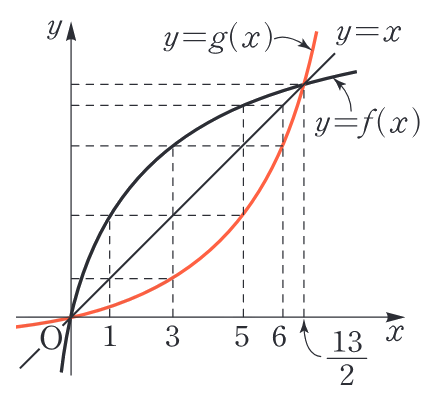
\includegraphics[width=\dmfigw]{figures/fig-244-575.png}\end{minipage}\par
